% Options for packages loaded elsewhere
\PassOptionsToPackage{unicode}{hyperref}
\PassOptionsToPackage{hyphens}{url}
%
\documentclass[
]{article}
\usepackage{amsmath,amssymb}
\usepackage{lmodern}
\usepackage{iftex}
\ifPDFTeX
  \usepackage[T1]{fontenc}
  \usepackage[utf8]{inputenc}
  \usepackage{textcomp} % provide euro and other symbols
\else % if luatex or xetex
  \usepackage{unicode-math}
  \defaultfontfeatures{Scale=MatchLowercase}
  \defaultfontfeatures[\rmfamily]{Ligatures=TeX,Scale=1}
\fi
% Use upquote if available, for straight quotes in verbatim environments
\IfFileExists{upquote.sty}{\usepackage{upquote}}{}
\IfFileExists{microtype.sty}{% use microtype if available
  \usepackage[]{microtype}
  \UseMicrotypeSet[protrusion]{basicmath} % disable protrusion for tt fonts
}{}
\makeatletter
\@ifundefined{KOMAClassName}{% if non-KOMA class
  \IfFileExists{parskip.sty}{%
    \usepackage{parskip}
  }{% else
    \setlength{\parindent}{0pt}
    \setlength{\parskip}{6pt plus 2pt minus 1pt}}
}{% if KOMA class
  \KOMAoptions{parskip=half}}
\makeatother
\usepackage{xcolor}
\IfFileExists{xurl.sty}{\usepackage{xurl}}{} % add URL line breaks if available
\IfFileExists{bookmark.sty}{\usepackage{bookmark}}{\usepackage{hyperref}}
\hypersetup{
  hidelinks,
  pdfcreator={LaTeX via pandoc}}
\urlstyle{same} % disable monospaced font for URLs
\usepackage{graphicx}
\makeatletter
\def\maxwidth{\ifdim\Gin@nat@width>\linewidth\linewidth\else\Gin@nat@width\fi}
\def\maxheight{\ifdim\Gin@nat@height>\textheight\textheight\else\Gin@nat@height\fi}
\makeatother
% Scale images if necessary, so that they will not overflow the page
% margins by default, and it is still possible to overwrite the defaults
% using explicit options in \includegraphics[width, height, ...]{}
\setkeys{Gin}{width=\maxwidth,height=\maxheight,keepaspectratio}
% Set default figure placement to htbp
\makeatletter
\def\fps@figure{htbp}
\makeatother
\setlength{\emergencystretch}{3em} % prevent overfull lines
\providecommand{\tightlist}{%
  \setlength{\itemsep}{0pt}\setlength{\parskip}{0pt}}
\setcounter{secnumdepth}{-\maxdimen} % remove section numbering
\ifLuaTeX
  \usepackage{selnolig}  % disable illegal ligatures
\fi

\author{}
\date{}

\begin{document}

\hypertarget{header-n0}{%
\section{Solubility lab}\label{header-n0}}

\hypertarget{header-n3}{%
\subsection{Procedure}\label{header-n3}}

Into a beaker of known weight was added an amount of salt, and the
beaker was then weighed. The mass of the salt was 4.0 grams. Water was
then gradually poured into the beaker until it covered the salt,
whereupon the solution was stirred until the salt stopped dissolving.
Water was then added repeatedly, in decreasing volume, to the beaker,
stirring in between, until the salt just barely dissolved in the water.
The final mass of water required to dissolve the salt was found to be
18.4 grams.

\hypertarget{header-n6}{%
\subsection{Photo}\label{header-n6}}

\begin{figure}
\centering
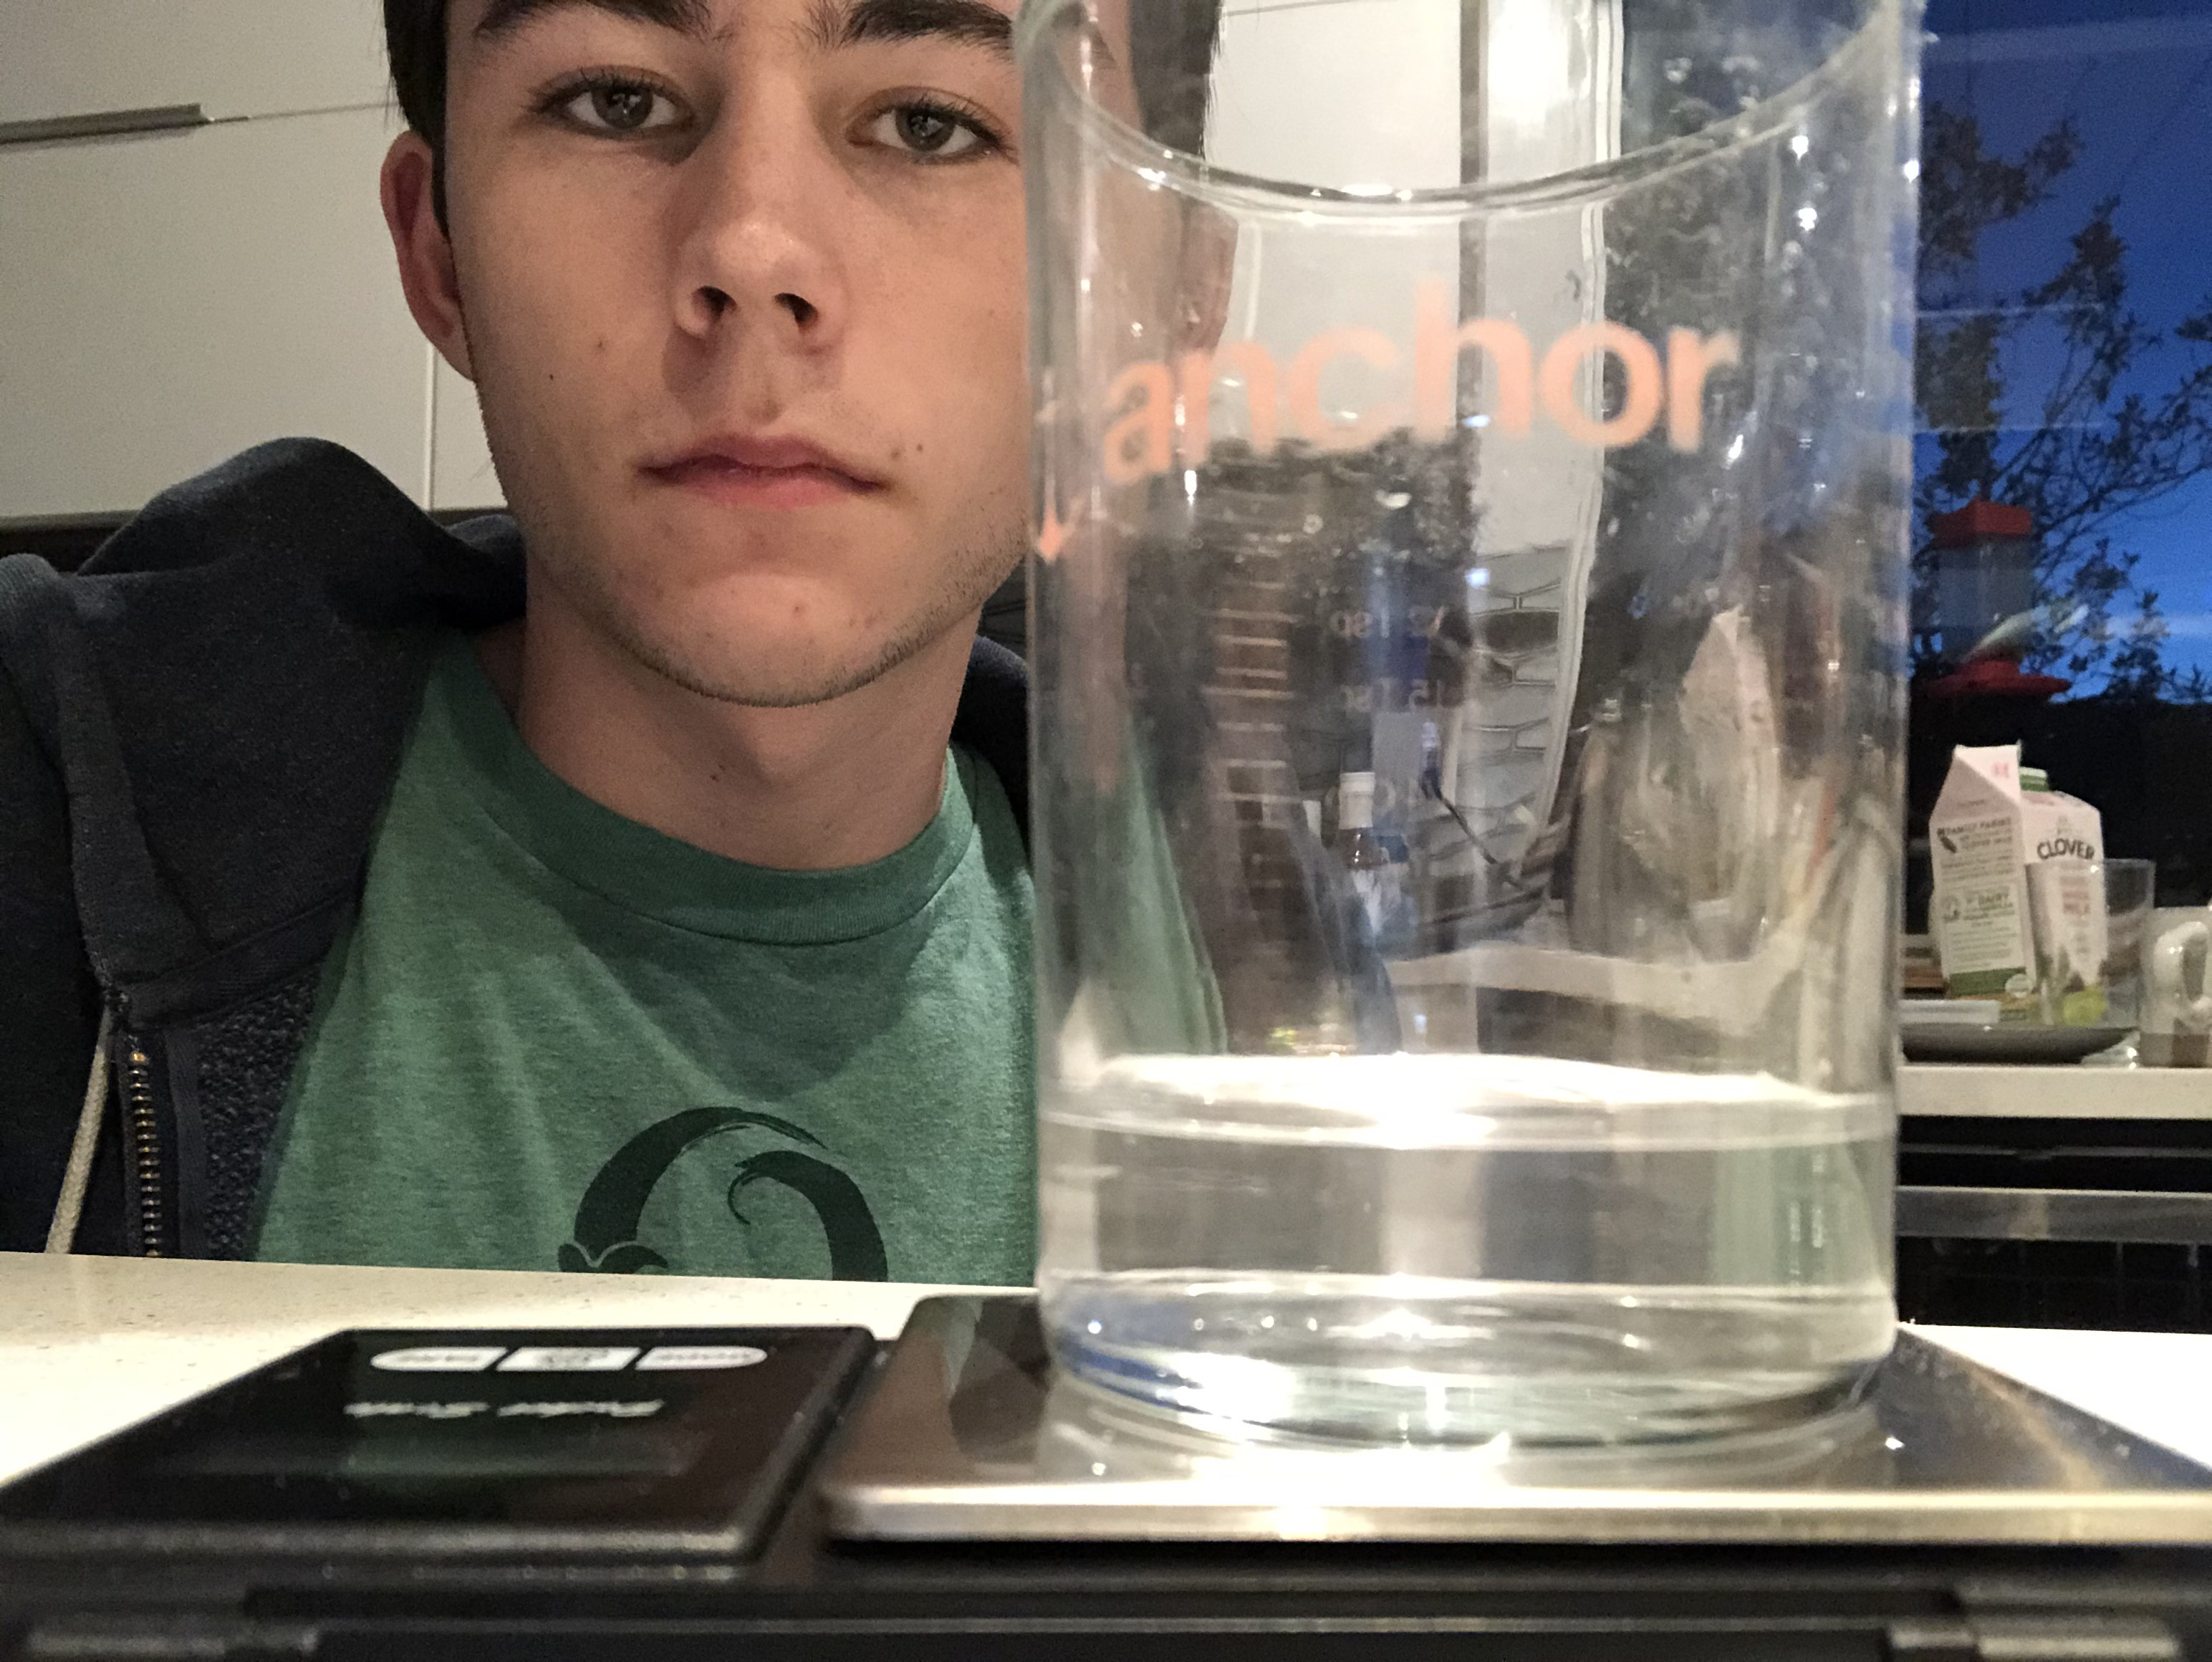
\includegraphics{/home/benh/Documents/School/Year4/Semester2/Chem/images/selfie_solubility.gif}
\caption{}
\end{figure}

\hypertarget{header-n9}{%
\subsection{Data}\label{header-n9}}

Salt: 4.0 g\\
Water: 18.4 mL

salt molar mass = 22.99 g/mol + 35.45 g/mol\\
salt molar mass = 58.44 g/mol

n = 4.0 g / 58.44 g/mol\\
n = 0.06845 mol

conc. = 0.06845 mol / 0.0184 L\\
conc. = 3.720 M

k = {[}p{]}\^{}c\emph{p / {[}r{]}\^{}c}r\\
k = (3.720 M) * (3.720 M)\\
k = 14

\end{document}
